\documentclass[a4paper, 12pt]{article}
\usepackage[utf8]{inputenc}
\usepackage[T1]{fontenc}
\usepackage[top=2.5cm, bottom=2.5cm, left=3cm, right=2.5cm]{geometry}
\usepackage{graphicx}
\usepackage{nopageno}
\usepackage{setspace}
\usepackage{amsmath}
\usepackage{titlesec}
\usepackage{array}
\usepackage{booktabs}
\usepackage{multirow}
\usepackage{float}
\usepackage{url}
\IfFileExists{newtxtext.sty}{%
    \usepackage{newtxtext,newtxmath}%
}{%
    \usepackage{mathptmx}%
}
\usepackage{multicol}
\usepackage[labelsep=period,skip=4pt]{caption}
\usepackage{indentfirst}
\usepackage{enumitem}
\usepackage{longtable}
\usepackage{tabularx}
\usepackage{siunitx}
\usepackage{pgfplots}
\usepackage{tikz}
\usepackage{xcolor}
\usepackage{listings}
\usepackage{hyperref}

\pgfplotsset{compat=1.16}
\usetikzlibrary{arrows.meta,positioning,calc}
\sisetup{
    output-decimal-marker={,},
    group-separator={.},
    group-digits=integer,
    range-phrase={--},
    range-units=single,
    detect-all,
    per-mode=symbol
}
\hypersetup{
    colorlinks=true,
    linkcolor=black,
    citecolor=black,
    urlcolor=black,
    hypertexnames=false,
    pdftitle={Laporan Audit Instrumentasi Group I - FIT310},
    pdfauthor={Group I}
}

% 1. Paragraph & spacing setting (Template O2)
\linespread{1.25}
\setlength{\parindent}{0.8cm}
\setstretch{1.25}
\setlength{\columnsep}{10pt}
\setlength{\parskip}{0pt}

\setlength{\textfloatsep}{6pt}
\setlength{\intextsep}{6pt}
\setlength{\floatsep}{6pt}

\titlespacing*{\section}{0pt}{8pt}{4pt}
\titlespacing*{\subsection}{0pt}{0.4em}{0.2em}
\titlespacing*{\subsubsection}{0pt}{0.3em}{0.15em}

\setlist[enumerate]{
    itemsep=2pt,
    parsep=0pt,
    topsep=0pt,
    partopsep=0pt
}
\setlist[itemize]{
    itemsep=2pt,
    parsep=0pt,
    topsep=0pt,
    partopsep=0pt
}

% 2. Figure and Table Setting
\renewcommand{\figurename}{Gambar}
\renewcommand{\tablename}{Tabel}

% 3. Pengaturan Section (Polosan, tanpa huruf/nomor) - Template O2
\renewcommand{\thesection}{}
\titleformat{\section}
{\normalfont\bfseries}{}{0pt}{}

% 4. Pengaturan Subsection (Format: a. Judul) - Template O2
\renewcommand{\thesubsection}{\alph{subsection}.}
\titleformat{\subsection}
{\normalfont\bfseries}{\thesubsection}{0.5em}{}

\renewcommand{\thesubsubsection}{}
\titleformat{\subsubsection}
{\normalfont\bfseries}{}{0pt}{}

% 5. Listing kode untuk Lampiran
\lstset{
    basicstyle=\ttfamily\footnotesize,
    breaklines=true,
    frame=single,
    columns=fullflexible,
    keepspaces=true,
    showstringspaces=false,
    xleftmargin=0.2cm
}

% 6. Makro metrologi
\newcommand{\uc}{u_{c}}
\newcommand{\uA}{u_{A}}
\newcommand{\uB}{u_{B}}
\newcommand{\dd}{\mathrm{d}}

% 7. Pustaka / Bibliografi (Template O2)
\usepackage{csquotes}
\IfFileExists{biblatex.sty}{%
    \usepackage[style=apa,sortcites=true,sorting=nyt,backend=biber]{biblatex}
    \DeclareLanguageMapping{american}{american-apa}
    \addbibresource{Pustaka.bib}
    \setlength{\bibitemsep}{0.0\baselineskip}
}{%
    \usepackage[numbers,sort&compress]{natbib}
    \bibliographystyle{apalike}
    \renewcommand{\bibsection}{}
    \setlength{\bibsep}{2pt}
    \newcommand{\printbibliography}[1][]{\footnotesize\bibliography{Pustaka}}
    \providecommand{\parencite}{\citep}
}

\sisetup{
    output-decimal-marker={.},
    group-separator={,},
    group-digits=integer,
    range-phrase={--},
    range-units=single,
    detect-all,
    per-mode=symbol
}
\hypersetup{
    pdftitle={Instrumentation Calibration and Metrological Evaluation Report - Universitas Airlangga},
    pdfauthor={Group I - Department of Physics, Universitas Airlangga}
}

\begin{document}
\renewcommand{\figurename}{Figure}
\renewcommand{\tablename}{Table}

    \begin{titlepage}
    \begin{center}
        % Title
        \textbf{INSTRUMENTATION CALIBRATION AND METROLOGICAL EVALUATION REPORT}\\[0.0\baselineskip]
        \textbf{CASE-BASED ELABORATIVE PROJECT IN PHYSICS MEASUREMENT}\\[0.0\baselineskip]
        \textbf{``ACCURACY AND UNCERTAINTY IN EXPERIMENTAL LABORATORY PRACTICE''}\\[0.0\baselineskip]
        \textbf{PAIRED EXPERIMENTS P1 (DENSITY) AND M3 (ENERGY)}\\[0.5\baselineskip]

        % Ruler
        \hrule height 2pt
        \vspace{0.5\baselineskip}

        % Course, Date, and Group
        {\footnotesize
        \begin{tabular*}{\textwidth}{@{\extracolsep{\fill}} l c r @{}}
            Course: Sensors and Measurement (FIT310) & Date: 17 November 2026 & Team: Group I
        \end{tabular*}
        }
        \vspace{2\baselineskip}

        \begin{figure}[H]
            \centering
            
\includegraphics[width=6cm, height=6cm]{Images/logo-unair.png}
        \end{figure}
        \vspace{1\baselineskip}

        \begin{table}[H]
            \centering
            \renewcommand{\arraystretch}{1.05}{
                \begin{tabular}{lc}
                    \multicolumn{2}{c}{\textbf{Prepared By (Group I)}} \\
                    Muhammad Abiyu Khansa & (182241036) \\
                    Farras Atha Pandita & (182241040) \\
                    Hendra Maulana & (182241043)
                \end{tabular}}
        \end{table}

        \textbf{Faculty Supervisors :} \\
        \centering
        Winarno, S.Si., M.T. (Sessions 1--7) \\
        Yhosep Gita Yhun Yhuwana, S.Si., M.T. (Sessions 8--14)

        \vfill
        \begin{center}
            \textbf{PHYSICS STUDY PROGRAM \\
                    DEPARTMENT OF PHYSICS \\
                    FACULTY OF SCIENCE AND TECHNOLOGY \\
                    UNIVERSITAS AIRLANGGA \\
                    2026}
        \end{center}
    \end{center}
\end{titlepage}

    \begin{center}
    \underline{\textbf{INSTRUMENTATION CALIBRATION AND METROLOGICAL EVALUATION:}} \\
    \underline{\textbf{ACCURACY AND UNCERTAINTY IN EXPERIMENTS}} \\
    \underline{\textbf{P1 (\textit{DENSITY}) AND M3 (\textit{ENERGY})}}
\end{center}

\begin{center}
    Muhammad Abiyu Khansa (182241036), Farras Atha Pandita (182241040), Hendra Maulana (182241043)
\end{center}

\hrule height 2pt

\begin{center}
    \textbf{Department of Physics, Faculty of Science and Technology, Universitas Airlangga, Surabaya}
\end{center}

\vspace{10pt}
\renewcommand{\abstractname}{\normalsize{ABSTRACT}}
\begin{abstract}
\noindent
This report presents the instrumentation calibration and metrological evaluation conducted by Group~I across two physics experiments: P1 (density of a brass cylinder) and M3 (conservation of mechanical energy on an inclined air track). In accordance with the three-member team protocol, each measurand was recorded across $n=8$ repeated trials. Outlier screening using the $3\sigma$ criterion retained all data points. Uncertainties were evaluated following ISO-GUM guidelines (Type~A, Type~B, combined $\uc$, and expanded $U$ at $k=2$). Experiment P1 yielded $\rho=(8.493\pm0.035)\ \si{g/cm^3}$, with the largest uncertainty contribution originating from diameter ($85\%$). Calibration of the digital balance against $8$ standard reference masses produced $y=0.999975\,x+0.0421\ \si{g}$ with $R^2\approx 1$; however, residual plotting revealed a systematic parabolic pattern (maximum deviation $0.032\ \si{g}$), demonstrating that $R^2$ alone is insufficient to establish linearity. Experiment M3 yielded $\Delta E=E_1-E_2=(-2.79\pm0.61)\times10^{-3}\ \si{J}$; the negative sign indicates a higher apparent final energy than initial energy, which is physically impossible in a dissipative system. This outcome is diagnosed as a systematic instrumentation error (primarily the photogate optoelectronic \textit{response time delay}) rather than a violation of energy conservation.
\end{abstract}

\vspace{5pt}
\noindent\textbf{Keywords:} instrumentation calibration, ISO-GUM, expanded uncertainty, OLS regression, residual analysis, density, energy conservation, air track.


%======== Main Body ===========
\newpage
\section{INTRODUCTION}
        \subsection{Background}
        The Basic Physics Laboratory received a new batch of instruments and sensors, including digital balances, vernier calipers, an air track equipped with motion sensors (photogates), oscilloscopes, and digital thermometers. When this batch was deployed across identical experiments by multiple student teams, distinct inter-instrument data deviations emerged. Such deviations may originate from mechanical hysteresis and friction, environmental disturbances (\textit{modifying inputs}), signal \textit{noise}, system \textit{loading effects}, or parallax and digital resolution errors \parencite{Bentley2005}.

        Under these conditions, our team served as the Instrumentation Calibration and Evaluation Team. The objective was to determine whether observed deviations stem from internal instrument defects, calibration errors, \textit{loading effects}, environmental disturbances, or random uncertainty \parencite{Yhuwana2026}. Group~I was assigned the paired experiments \textbf{P1 (\textit{Density})} and \textbf{M3 (\textit{Energy})}, focusing on static and dynamic measurement characteristics as well as motion sensor response. Because the group consists of three members, the number of repetitions was reduced by $25\%$ to $n=8$ per measurand without compromising analytical depth.

        \subsection{Problem Statements}
        The evaluation addresses four core questions:
        \begin{enumerate}
            \item What are the static and dynamic performance characteristics of the instruments used in experiments P1 and M3?
            \item What are the calibration results of the digital balance against standard reference masses, and does the residual distribution support true linearity?
            \item What are the combined uncertainty ($\uc$) and expanded uncertainty ($U$, $k=2$) for brass density $\rho$ and mechanical energy loss $\Delta E$?
            \item How do instrumental limitations affect scientific conclusions regarding material density and conservation of mechanical energy?
        \end{enumerate}

        \subsection{Objectives}
        \begin{enumerate}
            \item Map static and dynamic instrument performance parameters: \textit{measurand}, \textit{range}, resolution, sensitivity, accuracy, precision, \textit{repeatability}, linearity, \textit{response time}, stability, and \textit{noise} \parencite{JCGM2012VIM}.
            \item Perform structured calibration against traceable reference standards, fit an OLS model $y=ax+b$, and inspect residual plots.
            \item Compute $\uA$, $\uB$, $\uc$, and $U$ ($k=2$, $\approx 95\%$ confidence level) and apply ISO-GUM significant-figure rules \parencite{JCGM2008GUM}.
            \item Formulate a reflective \textit{``so what?''} interpretation and technical calibration recommendations.
        \end{enumerate}

        \subsection{Instrument Specifications}
        The evaluated instruments and specifications used in the calculations are summarized in Table~\ref{tab:profil}.
%=== Instrument Profile Table (Full Width) ===
\begin{table}[H]
\centering
\singlespacing
\caption{Evaluated instrument specifications (Group I).}
\label{tab:profil}
\small
\begin{tabularx}{\textwidth}{@{}l l X l@{}}
\toprule
\textbf{Experiment} & \textbf{Instrument} & \textbf{\textit{Measurand}} & \textbf{Resolution}\\
\midrule
P1 & Digital balance (0--500 g) & Brass cylinder mass $m$ & \SI{0.01}{g}\\
P1 & Vernier caliper & Cylinder diameter $d$ and height $h$ & \SI{0.05}{mm}\\
M3 & Digital balance & \textit{Glider} mass $M$ & \SI{0.01}{g}\\
M3 & Vernier caliper & \textit{Flag} width $w$ & \SI{0.05}{mm}\\
M3 & Ruler / height gauge & Elevation difference $\Delta h$ & \SI{0.1}{mm}\\
M3 & Photogate + digital \textit{timer} & Interruption times $\Delta t_1$, $\Delta t_2$ & \SI{0.1}{ms}\\
Calibration & Class F2 standard weights & Reference mass $x$ (10--300 g) & $u_{\mathrm{std}}\le\SI{0.002}{g}$\\
\bottomrule
\end{tabularx}
\end{table}

\section{EXPERIMENTAL METHODS AND DATA}
        \subsection{Setup and Procedure for P1 (Density)}
        The density of the brass cylinder is determined indirectly from three measured quantities \parencite{HallidayResnickWalker}:
        \begin{equation}
            \rho=\frac{m}{V}=\frac{4m}{\pi d^{2}h}.
            \label{eq:rho}
        \end{equation}
        The procedure consists of: (1) zeroing the digital balance on a level, vibration-free surface; (2) measuring cylinder mass $n=8$ times; (3) measuring diameter and height $n=8$ times across varied positions with a vernier caliper; (4) screening data with the $3\sigma$ criterion; and (5) computing means and uncertainties before propagating them into $\rho$.

        \subsection{Setup and Procedure for M3 (Air-Track Energy)}
        A \textit{glider} of mass $M$ carrying an interrupter \textit{flag} of width $w$ slides down an inclined air track through two photogates (Figure~\ref{fig:skema}). Photogate~1 is positioned at $x_1=\SI{30}{cm}$ with reference elevation $\Delta h=\SI{28}{mm}$ above Photogate~2, which sits at $x_2=\SI{110}{cm}$ (track span $\Delta s=\SI{0.80}{m}$). Velocity at each gate is computed as:
        \begin{equation}
            v_i=\frac{w}{\Delta t_i},\qquad i=1,2,
            \label{eq:v}
        \end{equation}
        and total mechanical energy at each gate (local gravity $g=\SI{9.806}{m/s^2}$) is \parencite{HallidayResnickWalker}:
        \begin{equation}
            E_1=\tfrac{1}{2}Mv_1^{2}+Mg\,\Delta h,\qquad
            E_2=\tfrac{1}{2}Mv_2^{2},\qquad
            \Delta E=E_1-E_2.
            \label{eq:E}
        \end{equation}
        Under ideal conservative motion $\Delta E=0$, whereas friction and air drag should yield $\Delta E>0$.
%=== Experiment M3 Schematic (Full Width) ===
\begin{figure}[H]
\centering
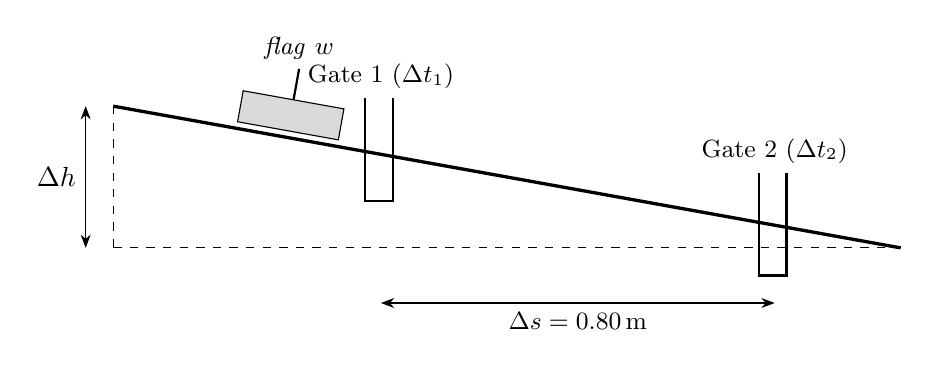
\begin{tikzpicture}[>=Stealth,scale=1.0]
  % inclined track
  \draw[very thick] (0,2.2) -- (10,0.4);
  \draw[dashed] (0,0.4) -- (10,0.4);
  \draw[dashed] (0,2.2) -- (0,0.4);
  \draw[<->] (-0.35,0.4) -- (-0.35,2.2) node[midway,left]{$\Delta h$};
  % glider
  \begin{scope}[rotate=-10.2,shift={(1.2,2.2)}]
    \fill[gray!30,draw=black] (0,0.05) rectangle (1.3,0.45);
    \draw[thick] (0.65,0.45) -- (0.65,0.85);
    \node[above] at (0.65,0.85) {\small \textit{flag} $w$};
  \end{scope}
  % gate 1
  \draw[thick] (3.2,2.3) -- (3.2,1.0) -- (3.55,1.0) -- (3.55,2.3);
  \node[above] at (3.4,2.3) {\small Gate 1 ($\Delta t_1$)};
  % gate 2
  \draw[thick] (8.2,1.35) -- (8.2,0.05) -- (8.55,0.05) -- (8.55,1.35);
  \node[above] at (8.4,1.35) {\small Gate 2 ($\Delta t_2$)};
  \draw[<->] (3.4,-0.3) -- (8.4,-0.3) node[midway,below]{\small $\Delta s=\SI{0.80}{m}$};
\end{tikzpicture}
\caption{Experimental setup for M3: \textit{glider} on an inclined air track passing through two photogates.}
\label{fig:skema}
\end{figure}

\subsection{Raw Datasets for P1 and M3 (\texorpdfstring{$n=8$}{n=8})}
        All raw observations for P1 (brass cylinder) and M3 (air track) were recorded without initial rounding, as listed in Table~\ref{tab:p1} and Table~\ref{tab:m3}.

        \subsection{Outlier Screening via \texorpdfstring{$3\sigma$}{3 sigma} Criterion}
        A data point is flagged as an outlier if $|x_i-\bar{x}|>3\sigma$ \parencite{Taylor1997}. Screening results across all quantities are given in Table~\ref{tab:z}. Every observation passed, so all $n=8$ trials were retained.

        Notably, for small samples, this criterion cannot mathematically flag an outlier when $\sigma$ is estimated from the sample itself. The maximum possible standardized deviation is $(n-1)/\sqrt{n}=7/\sqrt{8}\approx 2.47$ sample standard deviations, which is strictly below $3$. Passing all points is therefore not conclusive proof of outlier-free data; rather, data integrity is supported by the small standard deviations and visual consistency.
%=== Raw Data Tables (Full Width) ===
\begin{table}[H]
\centering
\singlespacing
\caption{Raw dataset for P1 (brass cylinder, $n=8$) with $3\sigma$ screening status.}
\label{tab:p1}
\small
\begin{tabular}{c S[table-format=2.2] c S[table-format=2.2] c S[table-format=2.2] c}
\toprule
\textbf{Trial} & {\textbf{Mass (g)}} & \textbf{Status} & {\textbf{Diameter (mm)}} & \textbf{Status} & {\textbf{Height (mm)}} & \textbf{Status} \\
\midrule
1 & 67.22 & Pass & 20.05 & Pass & 25.10 & Pass \\
2 & 67.21 & Pass & 20.00 & Pass & 25.15 & Pass \\
3 & 67.23 & Pass & 20.05 & Pass & 25.10 & Pass \\
4 & 67.20 & Pass & 20.10 & Pass & 25.05 & Pass \\
5 & 67.24 & Pass & 20.00 & Pass & 25.10 & Pass \\
6 & 67.22 & Pass & 20.05 & Pass & 25.15 & Pass \\
7 & 67.21 & Pass & 20.00 & Pass & 25.10 & Pass \\
8 & 67.23 & Pass & 20.05 & Pass & 25.05 & Pass \\
\bottomrule
\end{tabular}
\end{table}

\begin{table}[H]
\centering
\singlespacing
\caption{Raw dataset for M3 (air track, $n=8$) with $3\sigma$ screening status.}
\label{tab:m3}
\small
\begin{tabular}{c S[table-format=1.4] c S[table-format=1.4] c S[table-format=3.2] S[table-format=2.2] S[table-format=2.1]}
\toprule
\textbf{Trial} & {$\Delta t_1$ (s)} & \textbf{Status} & {$\Delta t_2$ (s)} & \textbf{Status} & {$M$ (g)} & {$w$ (mm)} & {$\Delta h$ (mm)} \\
\midrule
1 & 0.0521 & Pass & 0.0278 & Pass & 200.10 & 25.00 & 28.0 \\
2 & 0.0519 & Pass & 0.0279 & Pass & 200.12 & 25.05 & 28.1 \\
3 & 0.0523 & Pass & 0.0277 & Pass & 200.08 & 25.00 & 28.0 \\
4 & 0.0520 & Pass & 0.0280 & Pass & 200.11 & 24.95 & 27.9 \\
5 & 0.0522 & Pass & 0.0278 & Pass & 200.09 & 25.00 & 28.0 \\
6 & 0.0518 & Pass & 0.0279 & Pass & 200.10 & 25.05 & 28.1 \\
7 & 0.0524 & Pass & 0.0277 & Pass & 200.13 & 25.00 & 28.0 \\
8 & 0.0521 & Pass & 0.0278 & Pass & 200.07 & 24.95 & 27.9 \\
\bottomrule
\end{tabular}
\end{table}


%=== Z-max Screening Table (Full Width) ===
\begin{table}[H]
\centering
\singlespacing
\caption{Maximum standardized deviation from the mean ($z_{\max}=\max|x_i-\bar{x}|/s$).}
\label{tab:z}
\small
\begin{tabular}{l c c}
\toprule
\textbf{Quantity} & $z_{\max}$ & \textbf{Result ($z_{\max}<3$)}\\
\midrule
Mass $m$ (P1) & 1.53 & All pass\\
Diameter $d$ & 1.77 & All pass\\
Height $h$ & 1.32 & All pass\\
Time $\Delta t_1$ & 1.50 & All pass\\
Time $\Delta t_2$ & 1.69 & All pass\\
\textit{Glider} mass $M$ & 1.50 & All pass\\
\textit{Flag} width $w$ & 1.32 & All pass\\
Elevation $\Delta h$ & 1.32 & All pass\\
\bottomrule
\end{tabular}
\end{table}

\section{INSTRUMENT CHARACTERISTIC ANALYSIS}
        \subsection{Summary of Static and Dynamic Parameters}
        Table~\ref{tab:param} summarizes the metrological performance metrics determined from the evaluation data \parencite{JCGM2012VIM,MorrisLangari}. Unmeasured datasheet assumptions are explicitly noted.
%=== Metrological Performance Summary Table (Full Width) ===
\begin{table}[H]
\centering
\singlespacing
\caption{Metrological performance parameters of the digital balance and motion sensors.}
\label{tab:param}
\small
\begin{tabularx}{\textwidth}{@{}l l X@{}}
\toprule
\textbf{Parameter} & \textbf{Category} & \textbf{Evaluation Result}\\
\midrule
\textit{Measurand} & Static/Dynamic & Mass (g), length (mm), interruption time (s)\\
\textit{Range} & Static & Balance \SIrange{0}{500}{g}; vernier caliper \SIrange{0}{150}{mm}\\
Resolution & Static & Balance \SI{0.01}{g}; caliper \SI{0.05}{mm}; \textit{timer} \SI{0.1}{ms}\\
Sensitivity & Static & $S=a=0.999975\ \si{g/g}$ (ideal $1.000000$)\\
Accuracy & Static & Mean bias $\bar{m}-m_{\mathrm{ref}}=\SI{0.020}{g}$ ($0.030\%$) vs. \SI{67.20}{g} reference\\
Precision & Static & $s_m=\SI{0.0131}{g}$ ($n=8$)\\
\textit{Repeatability} & Static & $r=2.8\,s_r=\SI{0.037}{g}$\\
Linearity & Static & Max. deviation from OLS $\SI{0.032}{g}$ ($0.011\%$ of \SI{300}{g} FS); curved residuals\\
\textit{Response time} & Dynamic & Photogate optoelectronic delay $\tau\approx\SI{0.8}{ms}$ (\textit{rise} $\approx\SI{20}{\micro s}$, \textit{fall} $\approx\SI{35}{\micro s}$); datasheet assumption used in analysis, pending oscilloscope verification\\
Stability & Static/Dynamic & Balance \textit{zero drift} $+\SI{0.03}{g}$ over $30$ min (Table~\ref{tab:drift})\\
\textit{Noise} & Static/Dynamic & Random balance fluctuation $s_m=\SI{0.013}{g}$ ($\approx 1$ resolution digit)\\
\bottomrule
\end{tabularx}
\end{table}

\subsection{Static Characteristics (Experiment P1)}
            \subsubsection{Accuracy and Error}
            With $E_m=\bar{m}=\SI{67.22}{g}$ and reference $E_o=\SI{67.20}{g}$:
            \begin{align}
                E_{\mathrm{abs}} &= |E_m-E_o|=\SI{0.020}{g},\\
                E_{\mathrm{rel}} &= \frac{|E_m-E_o|}{E_o}=2.98\times10^{-4},\\
                \%E &= 0.030\%.
            \end{align}
            This bias equals twice the balance resolution. Because $E_{\mathrm{abs}}=\SI{0.020}{g}$ exceeds the expanded mass uncertainty $U_m=\SI{0.011}{g}$, the bias is metrologically significant and aligns with the calibration offset observed in OLS modeling.

            \subsubsection{Repeatability and Zero Drift}
            The sample standard deviation $s_r=\SI{0.0131}{g}$ yields a repeatability limit $r=2.8\,s_r=\SI{0.037}{g}$. No-load \textit{zero drift} measurements following cyclic loading are listed in Table~\ref{tab:drift}.

            A zero shift of $+\SI{0.03}{g}$ over $30$ minutes ($\approx\SI{1e-3}{g/min}$) corresponds to three resolution steps, attributable to load-cell mechanical \textit{creep} (\textit{strain gauge}) and thermal amplifier/ADC drift. In practice, the balance should be re-zeroed (\textit{tare}) before each measurement run \parencite{MorrisLangari}.

        \subsection{Dynamic Characteristics and Loading Effects (Experiment M3)}
            \subsubsection{Photogate Response Time Delay}
            Comparator hysteresis inside the photogate introduces a latency $\tau$, modeled as $\Delta t_{\mathrm{meas}}=\Delta t_{\mathrm{true}}-\tau$, which inflates measured velocities. Using $\tau=\SI{0.8}{ms}$ and mean times $\overline{\Delta t_1}=\SI{52.10}{ms}$ and $\overline{\Delta t_2}=\SI{27.825}{ms}$ yields Table~\ref{tab:delay}.

            The relative bias at Gate~2 is nearly double that at Gate~1 because its shorter interruption time magnifies the fixed ratio $\tau/\Delta t$. This illustrates a hallmark of systematic error: increasing sample repetitions cannot reduce it \parencite{Taylor1997}.

            \subsubsection{Loading Effect and Th\'evenin Equivalent}
            System loading is framed using a Th\'evenin equivalent model \parencite{Bentley2005}:
            \begin{equation}
                \frac{E_m}{E_o}=\frac{R_m}{R_{AB}+R_m}.
                \label{eq:thevenin}
            \end{equation}
            Achieving $E_m/E_o\approx1$ requires $R_m\gg R_{AB}$ (e.g., $R_m\ge 99\,R_{AB}$ for $<1\%$ loading error). On the air track, mechanical boundary-layer drag and passive eddy-current damping act analogously to internal impedance $R_{AB}$ that dissipates energy. Equation~\eqref{eq:thevenin} serves here as a conceptual framework rather than a quantitative model since mechanical $R_{AB}$ was not directly measured.

            \subsubsection{Modifying Inputs}
            Air currents from laboratory HVAC vents alter aerodynamic drag on the \textit{glider}, while slight track-level non-uniformity modifies the effective $\Delta h$. Both represent environmental \textit{modifying inputs} rather than intrinsic sensor defects \parencite{Bentley2005}.
%=== Zero Drift & Delay Tables (Full Width) ===
\begin{table}[H]
\centering
\singlespacing
\caption{No-load digital balance \textit{zero drift} test.}
\label{tab:drift}
\small
\begin{tabular}{l *{7}{S[table-format=1.2]}}
\toprule
Time (min) & {0} & {5} & {10} & {15} & {20} & {25} & {30}\\
Zero reading (g) & 0.00 & 0.00 & 0.01 & 0.01 & 0.02 & 0.02 & 0.03\\
\bottomrule
\end{tabular}
\end{table}

\begin{table}[H]
\centering
\singlespacing
\caption{Impact of photogate \textit{response time delay} ($\tau=\SI{0.8}{ms}$) on velocity.}
\label{tab:delay}
\small
\begin{tabular}{l S[table-format=1.4] S[table-format=1.4] S[table-format=1.2]}
\toprule
\textbf{Gate} & {$v_{\mathrm{meas}}$ (m/s)} & {$v_{\mathrm{corr}}$ (m/s)} & {Bias (\%)}\\
\midrule
1 & 0.4798 & 0.4726 & 1.54\\
2 & 0.8985 & 0.8734 & 2.88\\
\bottomrule
\end{tabular}
\end{table}

\section{UNCERTAINTY AND ERROR PROPAGATION}
        \subsection{ISO-GUM Formulation}
        Type~A ($\uA$), Type~B ($\uB$), combined ($\uc$), and expanded ($U$) uncertainties follow ISO-GUM standards \parencite{JCGM2008GUM}:
        \begin{align}
            \uA &= \frac{s}{\sqrt{n}},\quad s=\sqrt{\frac{\sum_{i=1}^{n}(x_i-\bar{x})^2}{n-1}},\label{eq:uA}\\
            \uB &= \frac{\text{Resolution}}{2\sqrt{3}},\label{eq:uB}\\
            \uc &= \sqrt{\uA^{2}+\uB^{2}},\quad U=k\,\uc=2\,\uc.\label{eq:U}
        \end{align}
        For a derived measurand $f(x_1,\dots,x_N)$, first-order uncertainty propagation is applied:
        \begin{equation}
            \uc(f)=\sqrt{\sum_{i=1}^{N}\left(\frac{\partial f}{\partial x_i}\right)^{2}\uc^{2}(x_i)}.
            \label{eq:prop}
        \end{equation}
        Final values report $U$ rounded to two significant figures, with the mean rounded to match the last decimal place of $U$.

        \subsection{Direct Measurand Uncertainties in P1}
        Direct measurement uncertainties for P1 are listed in Table~\ref{tab:uP1}, giving:
        \begin{align*}
            m &= (67.220\pm0.011)\ \si{g},\\
            d &= (2.0038\pm0.0038)\ \si{cm},\\
            h &= (2.5100\pm0.0039)\ \si{cm}.
        \end{align*}

        \subsection{Propagation to Brass Density \texorpdfstring{$\rho$}{rho}}
        From Equation~\eqref{eq:rho}, the relative combined uncertainty is:
        \begin{equation}
            \frac{\uc(\rho)}{\rho}=\sqrt{\left(\frac{\uc(m)}{m}\right)^{2}+4\left(\frac{\uc(d)}{d}\right)^{2}+\left(\frac{\uc(h)}{h}\right)^{2}}.
            \label{eq:urho}
        \end{equation}
        The factor of $4$ arises from $d^2$ in the denominator. The uncertainty budget is detailed in Table~\ref{tab:budget}.

        With cylinder volume $V=\tfrac{\pi}{4}d^2h=\SI{7.9150}{cm^3}$, we obtain $\rho=\SI{8.4927}{g/cm^3}$, $\uc(\rho)=\SI{0.0175}{g/cm^3}$, and $U(\rho)=\SI{0.0350}{g/cm^3}$:
        \begin{equation}
            \boxed{\rho=(8.493\pm0.035)\ \si{g/cm^3}\quad(k=2),\qquad \frac{U}{\rho}=0.41\%.}
        \end{equation}
        This matches standard brass densities ($\approx 8.4\text{--}8.7\ \si{g/cm^3}$ depending on Cu--Zn ratio), though a $0.41\%$ relative band cannot distinguish specific brass alloys. Because diameter contributes $85\%$ of variance, replacing the vernier caliper (\SI{0.05}{mm}) with a micrometer (\SI{0.01}{mm}) is the highest-impact upgrade.
%=== P1 Uncertainty & Budget Tables (Full Width) ===
\begin{table}[H]
\centering
\singlespacing
\caption{Uncertainty evaluation of direct measurands in P1 ($n=8$).}
\label{tab:uP1}
\small
\begin{tabular}{l S[table-format=2.5] S[table-format=1.5] S[table-format=1.5]}
\toprule
\textbf{Parameter} & {Mass (g)} & {Diameter (cm)} & {Height (cm)}\\
\midrule
Mean $\bar{x}$ & 67.22000 & 2.00375 & 2.51000\\
Std. deviation $s$ & 0.01309 & 0.00354 & 0.00378\\
$\uA=s/\sqrt{n}$ & 0.00463 & 0.00125 & 0.00134\\
Resolution $\Delta x$ & 0.01000 & 0.00500 & 0.00500\\
$\uB=\Delta x/(2\sqrt{3})$ & 0.00289 & 0.00144 & 0.00144\\
$\uc$ & 0.00546 & 0.00191 & 0.00197\\
$U=2\uc$ & 0.01091 & 0.00382 & 0.00393\\
\bottomrule
\end{tabular}
\end{table}

\begin{table}[H]
\centering
\singlespacing
\caption{Uncertainty budget for brass density $\rho$.}
\label{tab:budget}
\small
\begin{tabular}{l S[table-format=1.5] S[table-format=1.5] S[table-format=3.1]}
\toprule
\textbf{Source} & {$\uc(x)/x$} & {Contribution to $\uc(\rho)/\rho$} & {Variance share (\%)}\\
\midrule
Mass $m$ & 0.00008 & 0.00008 & 0.2\\
Diameter $d$ ($\times2$) & 0.00095 & 0.00191 & 85.4\\
Height $h$ & 0.00078 & 0.00078 & 14.4\\
\midrule
\textbf{Combined} & & 0.00206 & 100.0\\
\bottomrule
\end{tabular}
\end{table}

\subsection{Direct Measurand Uncertainties in M3}
        Direct measurand uncertainties for M3 are given in Table~\ref{tab:uM3}. Velocities from Equation~\eqref{eq:v} with $\uc(v)/v=\sqrt{(\uc(w)/w)^2+(\uc(\Delta t)/\Delta t)^2}$ are:
        \begin{align*}
            v_1 &= (0.4798\pm0.0016)\ \si{m/s},\\
            v_2 &= (0.8985\pm0.0033)\ \si{m/s}.
        \end{align*}

        \subsection{Propagation to Mechanical Energy and \texorpdfstring{$\Delta E$}{Delta E}}
        Because $E_1$ and $E_2$ share $M$ and $w$, they are correlated. Consequently, $\uc(\Delta E)$ is propagated directly from the combined expression:
        \begin{equation}
            \Delta E=M\left[\tfrac{1}{2}w^{2}\left(\frac{1}{\Delta t_1^{2}}-\frac{1}{\Delta t_2^{2}}\right)+g\,\Delta h\right]
            \label{eq:dEfull}
        \end{equation}
        via Equation~\eqref{eq:prop} with respect to $M$, $w$, $\Delta t_1$, $\Delta t_2$, and $\Delta h$ (results in Table~\ref{tab:E}).

        Treating $E_1$ and $E_2$ as independent gives $U(\Delta E)=\SI{0.00064}{J}$, nearly identical to the correlated value $\SI{0.00061}{J}$. The dominant uncertainty contributor is $\Delta t_2$ ($\approx 80\%$ of variance), followed by $w$, $\Delta h$, and $\Delta t_1$, while $M$ is negligible.

        \subsection{Final Reporting and Significant Figures}
        Following ISO-GUM rules, the final reported results are $\rho=(8.493\pm0.035)\ \si{g/cm^3}$ and $\Delta E=(-2.8\pm0.6)\times10^{-3}\ \si{J}$.
%=== M3 Uncertainty & Energy Tables (Full Width) ===
\begin{table}[H]
\centering
\singlespacing
\caption{Uncertainty evaluation of direct measurands in M3 ($n=8$).}
\label{tab:uM3}
\small
\begin{tabular}{l S[table-format=1.6] S[table-format=1.2e-1] S[table-format=1.2e-1] S[table-format=1.2e-1]}
\toprule
\textbf{Quantity} & {Mean} & {$\uA$} & {$\uB$} & {$\uc$}\\
\midrule
$\Delta t_1$ (s) & 0.052100 & 7.07e-5 & 2.89e-5 & 7.64e-5\\
$\Delta t_2$ (s) & 0.027825 & 3.66e-5 & 2.89e-5 & 4.66e-5\\
$M$ (kg) & 0.200100 & 7.07e-6 & 2.89e-6 & 7.64e-6\\
$w$ (m) & 0.025000 & 1.34e-5 & 1.44e-5 & 1.97e-5\\
$\Delta h$ (m) & 0.028000 & 2.67e-5 & 2.89e-5 & 3.93e-5\\
\bottomrule
\end{tabular}
\end{table}

\begin{table}[H]
\centering
\singlespacing
\caption{Mechanical energy and energy discrepancy ($k=2$).}
\label{tab:E}
\small
\begin{tabular}{l l}
\toprule
\textbf{Quantity} & \textbf{Result}\\
\midrule
$E_{k1}=\tfrac{1}{2}Mv_1^2$ & \SI{0.02304}{J}\\
$E_{p1}=Mg\Delta h$ & \SI{0.05494}{J}\\
$E_1=E_{k1}+E_{p1}$ & $(0.07798\pm0.00022)\ \si{J}$\\
$E_2=\tfrac{1}{2}Mv_2^2$ & $(0.08077\pm0.00060)\ \si{J}$\\
$\Delta E=E_1-E_2$ & $(-2.79\pm0.61)\times10^{-3}\ \si{J}$\\
\bottomrule
\end{tabular}
\end{table}

\section{CALIBRATION PROCEDURE AND VALIDATION}
        \subsection{Calibration Procedure}
        The digital balance was calibrated against Class F2 reference weights ($u_{\mathrm{std}}\le\SI{0.002}{g}$), providing reference accuracy one order better than balance resolution \parencite{Yhuwana2026}. Eight reference points spanning \SIrange{10}{300}{g} were measured and modeled via OLS linear regression $y=ax+b$:
        \begin{equation}
            a=\frac{n\sum x_iy_i-\sum x_i\sum y_i}{n\sum x_i^{2}-\left(\sum x_i\right)^{2}},\quad
            b=\frac{\sum y_i-a\sum x_i}{n}.
            \label{eq:ols}
        \end{equation}

        \subsection{Regression Results}
        Calibration points and residuals are tabulated in Table~\ref{tab:cal}. The OLS fit gives:
        \begin{equation}
            \boxed{y=0.999975\,x+0.0421\ \si{g},\qquad R^{2}=0.99999997.}
        \end{equation}
        The standard error of regression is $s_{y/x}=\SI{0.0217}{g}$, with slope uncertainty $u(a)=7.6\times10^{-5}$ and intercept uncertainty $u(b)=\SI{0.013}{g}$. Since $|a-1|=2.5\times10^{-5}<u(a)$, \textbf{balance sensitivity does not differ significantly from unity}. Intercept $b=\SI{0.042}{g}$ ($\approx 3.3\,u(b)$) matches the observed \textit{zero drift} (\SI{0.03}{g}), consistent with a zero-offset bias.
%=== OLS Calibration Table (Full Width) ===
\begin{table}[H]
\centering
\singlespacing
\caption{Digital balance calibration data, OLS model predictions, and residuals.}
\label{tab:cal}
\small
\begin{tabular}{c S[table-format=3.2] S[table-format=3.2] S[table-format=3.4] S[table-format=-1.4]}
\toprule
\textbf{Point} & {Standard $x$ (g)} & {Reading $y$ (g)} & {$\hat{y}$ (g)} & {$e_i=y_i-\hat{y}_i$ (g)}\\
\midrule
1 & 10.00 & 10.02 & 10.0419 & -0.0219\\
2 & 20.00 & 20.03 & 20.0416 & -0.0116\\
3 & 50.00 & 50.04 & 50.0409 & -0.0009\\
4 & 100.00 & 100.06 & 100.0396 & 0.0204\\
5 & 150.00 & 150.07 & 150.0384 & 0.0316\\
6 & 200.00 & 200.05 & 200.0371 & 0.0129\\
7 & 250.00 & 250.03 & 250.0359 & -0.0059\\
8 & 300.00 & 300.01 & 300.0346 & -0.0246\\
\bottomrule
\end{tabular}
\end{table}

\subsection{Residual Plot Analysis}
        Figure~\ref{fig:cal} shows the calibration curve and Figure~\ref{fig:res} displays its residuals. Residuals are \emph{not} randomly scattered around zero: signs switch only twice (three runs across eight points), positive in the middle range and negative at both extremes. A quadratic fit $y=c_2x^2+c_1x+c_0$ reduces the standard error from $\SI{0.0217}{g}$ to $\SI{0.0056}{g}$ with $c_2=-2.3\times10^{-6}\ \si{g^{-1}}$. Thus, even with $R^2=0.99999997\approx1$, \textbf{$R^2$ conceals systematic non-linear curvature} \parencite{Yhuwana2026}. The peak residual of $\SI{0.032}{g}$ is roughly three times the balance resolution.

        Gain error $y-x$ also varies non-uniformly ($+\SI{0.02}{g}$ at \SI{10}{g}, peaking at $+\SI{0.07}{g}$ at \SI{150}{g}, and dropping to $+\SI{0.01}{g}$ at \SI{300}{g}), reinforcing subtle elastic non-linearity in the load cell rather than a pure zero offset.
%=== Calibration and Residual Figures (Full Width) ===
\begin{figure}[H]
\centering
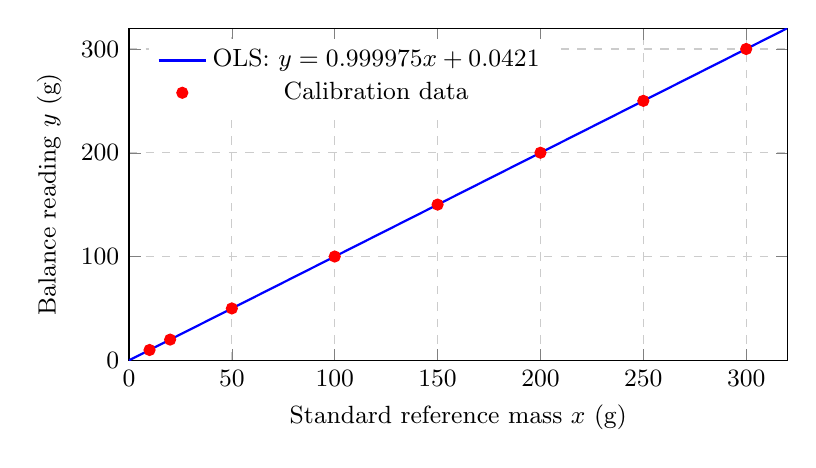
\begin{tikzpicture}
\begin{axis}[
  width=0.82\textwidth,height=5.8cm,
  xlabel={Standard reference mass $x$ (g)},ylabel={Balance reading $y$ (g)},
  xmin=0,xmax=320,ymin=0,ymax=320,
  grid=both,grid style={dashed,gray!40},
  legend pos=north west,legend style={font=\small,draw=none},
  tick label style={font=\small},label style={font=\small}]
\addplot[domain=0:320,samples=2,thick,blue]{0.999975*x+0.0421};
\addlegendentry{OLS: $y=0.999975x+0.0421$}
\addplot[only marks,mark=*,mark size=2pt,red]
  coordinates{(10,10.02)(20,20.03)(50,50.04)(100,100.06)(150,150.07)(200,200.05)(250,250.03)(300,300.01)};
\addlegendentry{Calibration data}
\end{axis}
\end{tikzpicture}
\caption{Digital balance calibration curve against standard masses. At full scale, data points and the OLS line appear superimposed, necessitating residual inspection.}
\label{fig:cal}
\end{figure}

\begin{figure}[H]
\centering
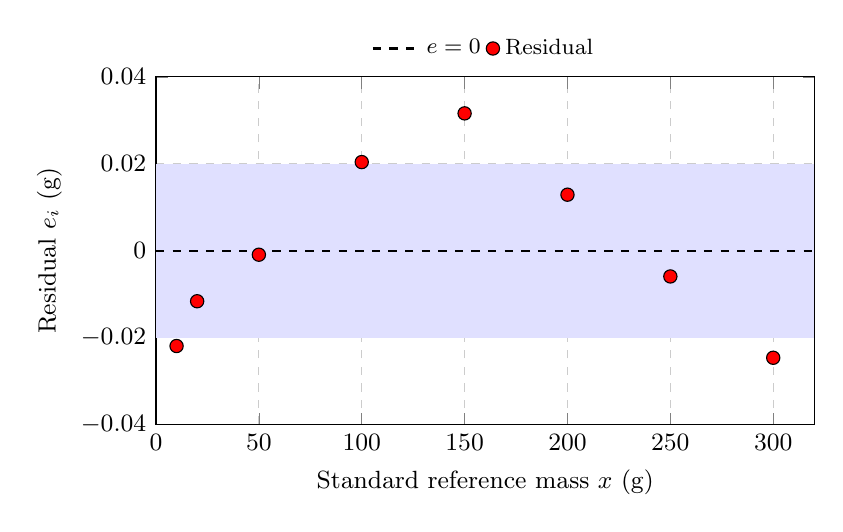
\begin{tikzpicture}
\begin{axis}[
  width=0.82\textwidth,height=6.0cm,
  xlabel={Standard reference mass $x$ (g)},ylabel={Residual $e_i$ (g)},
  xmin=0,xmax=320,ymin=-0.04,ymax=0.04,
  grid=both,grid style={dashed,gray!40},
  legend style={font=\footnotesize,draw=none,at={(0.5,1.02)},anchor=south,legend columns=-1},
  tick label style={font=\small},label style={font=\small},
  scaled y ticks=false,yticklabel style={/pgf/number format/fixed,/pgf/number format/precision=2}]
\fill[blue!12] (axis cs:0,-0.02) rectangle (axis cs:320,0.02);
\addplot[black,dashed,thick,domain=0:320,samples=2]{0};
\addplot[only marks,mark=*,mark size=2.4pt,red,draw=black]
  coordinates{(10,-0.0219)(20,-0.0116)(50,-0.0009)(100,0.0204)(150,0.0316)(200,0.0129)(250,-0.0059)(300,-0.0246)};
\legend{$e=0$,Residual}
\end{axis}
\end{tikzpicture}
\caption{Residual distribution relative to the OLS fit. The shaded band marks $\pm\SI{0.02}{g}$ ($\approx 2\times$ resolution). Four of eight points lie outside the band in a systematic $(-,-,-,+,+,+,-,-)$ inverted arc.}
\label{fig:res}
\end{figure}

\subsection{Five Validation Tests}
        A summary of the five instrument performance validation tests is presented in Table~\ref{tab:valid}.

        \subsection{Measurement Correction}
        When using the balance uncalibrated, true mass can be estimated via $x=(y-b)/a$. Across \SIrange{10}{300}{g}, this correction ranges from \SI{0.01}{g} to \SI{0.07}{g}—exceeding instrument resolution and warranted for precision work.
%=== Five Validation Tests Table (Full Width) ===
\begin{table}[H]
\centering
\singlespacing
\caption{Summary of the five instrument performance validation tests.}
\label{tab:valid}
\small
\begin{tabularx}{\textwidth}{@{}l X X@{}}
\toprule
\textbf{Test} & \textbf{Observed Result} & \textbf{Assessment}\\
\midrule
1. \textit{Accuracy} & P1 mass bias $\SI{0.020}{g}$ ($0.030\%$); max calibration error $+\SI{0.07}{g}$ at \SI{150}{g} ($0.047\%$) & Acceptable for lab use; bias $>U_m$ warrants correction\\
2. \textit{Repeatability} & $n=8$ (Group I): $s_r=\SI{0.0131}{g}$, $r=\SI{0.037}{g}$ & Good, $\approx 1$ resolution digit\\
3. \textit{Linearity} & Max deviation $\SI{0.032}{g}$ ($0.011\%$ FS); parabolic residual pattern & Practically linear, not purely random\\
4. \textit{Functional} & Zero function: no-load reading drifted from \SI{0.00}{g} to \SI{0.03}{g} over $30$ min (periodic re-zeroing needed). Gain: slope $a=0.999975$ ($2.5\times10^{-5}$ from unity). \textit{Display}: stable to $2$ decimals (\SI{0.01}{g}), trial spread $\le\SI{0.04}{g}$ ($67.20\text{--}\SI{67.24}{g}$) & Functional; requires periodic \textit{zeroing} (from drift, calibration, and repeatability data)\\
5. \textit{Response/stability} & \textit{Zero drift} $+\SI{0.03}{g}/30$ min; assumed photogate delay $\approx\SI{0.8}{ms}$ & Periodic \textit{tare} and latency correction required\\
\bottomrule
\end{tabularx}
\end{table}

\section{REFLECTIVE DISCUSSION AND INTEGRATION}
        \subsection{``So What?'' Analysis for Experiment P1}
        The result $\rho=(8.493\pm0.035)\ \si{g/cm^3}$ ($0.41\%$ relative uncertainty) reliably identifies the specimen as brass rather than pure copper or aluminum, though it cannot resolve exact Cu--Zn alloy grades. Since $85\%$ of variance originates from diameter, upgrading from a vernier caliper (\SI{0.05}{mm}) to a micrometer screw gauge (\SI{0.01}{mm}) reduces $U(\rho)$ from $\SI{0.035}{g/cm^3}$ to roughly $\SI{0.026}{g/cm^3}$ (changing $d$ alone), and to $\approx\SI{0.024}{g/cm^3}$ when applied to both $d$ and $h$—far more effective than adding mass repetitions.

        \subsection{``So What?'' Analysis for Experiment M3: Energy Conservation}
        Experiment M3 yielded $\Delta E=(-2.79\pm0.61)\times10^{-3}\ \si{J}$, differing from zero by $\approx 4.6\,U$. The negative sign ($E_2>E_1$) implies the \textit{glider} gained energy, which is physically impossible with friction and air drag. The sound scientific interpretation is neither ``energy conservation failed'' nor ``dissipation confirmed,'' but rather that \textbf{an uncorrected systematic error exceeds $U(\Delta E)$}.

        Candidate explanations and sufficiency checks:
        \begin{enumerate}
            \item \textbf{Response time delay.} Latency $\tau$ inflates $v_2$ more strongly than $v_1$ (Table~\ref{tab:delay}), overestimating $E_2$ relative to $E_1$. Applying $\tau=\SI{0.8}{ms}$ flips the discrepancy to $\Delta E=+\SI{0.97e-3}{J}$ (plausible positive dissipation), with $\Delta E=0$ occurring at $\tau\approx\SI{0.59}{ms}$. High sensitivity to $\tau$ confirms that latency must be measured directly rather than assumed.
            \item \textbf{Elevation error in $\Delta h$.} Explaining $\Delta E=0$ without $\tau$ correction would require $\Delta h\approx\SI{29.4}{mm}$ ($+\SI{1.4}{mm}$ above recorded, or $\approx 18\,U(\Delta h)$), unlikely as a sole cause, though track unevenness may contribute.
            \item \textbf{Flag width vs. instantaneous speed.} $v=w/\Delta t$ measures average speed across the interruption window rather than instantaneous midpoint speed on an accelerated track.
        \end{enumerate}
        With $\Delta E_{\text{corr}}\approx\SI{1e-3}{J}$ over $\Delta s=\SI{0.80}{m}$, the mean dissipative force is $\sim\SI{1e-3}{N}$, below the resolution threshold of current $U(\Delta E)$.

        \textbf{Implication:} random uncertainty ($U\approx\SI{6e-4}{J}$) is already small, yet dynamic systematic error dominates. Adding more trials will not fix the bias; direct sensor delay calibration is required.

        \subsection{Static vs. Dynamic Metrology Comparison}
        \begin{itemize}
            \item \textbf{Static (P1):} dominated by comparable random and resolution errors ($\uA \approx \uB$), mitigated via higher-resolution instruments. Balance non-linearity ($0.011\%$ FS) affects bias rather than $U(\rho)$.
            \item \textbf{Dynamic (M3):} dominated by systematic latency ($\tau$) scaled inversely by transit duration, becoming severe at higher speeds while evading $3\sigma$ outlier checks and sample standard deviations.
        \end{itemize}

    \section{CONCLUSIONS AND RECOMMENDATIONS}
        \subsection{Conclusions}
        \begin{enumerate}
            \item Brass cylinder density was determined as $\rho=(8.493\pm0.035)\ \si{g/cm^3}$ ($k=2$), with diameter accounting for $85\%$ of variance.
            \item Balance calibration gave $y=0.999975\,x+0.0421\ \si{g}$ ($R^2\approx 1$), yet parabolic residuals (max $\SI{0.032}{g}$) prove $R^2$ alone cannot confirm linearity.
            \item In M3, $\Delta E=(-2.79\pm0.61)\times10^{-3}\ \si{J}$ reflects systematic photogate latency rather than non-conservation. Correcting with $\tau=\SI{0.8}{ms}$ yields $\Delta E\approx+\SI{1.0e-3}{J}$, consistent with mild dissipation, pending direct $\tau$ measurement.
            \item Systematic dynamic errors escape variance-based checks and can only be resolved through calibration and compensation rather than additional repetitions.
        \end{enumerate}

        \subsection{Technical Recommendations}
        \begin{enumerate}
            \item \textbf{Measure photogate $\tau$} using an oscilloscope and microsecond-precision optical pulse source, then apply $\Delta t_{\mathrm{true}}=\Delta t_{\mathrm{meas}}+\tau$ in analysis software.
            \item \textbf{Use a micrometer screw gauge} for $d$ and $h$ in P1 to reduce the dominant contributor to $\rho$ uncertainty.
            \item \textbf{Level and verify the air track} with a precision spirit level (e.g., $\SI{0.02}{mm/m}$) and measure $\Delta h$ finer than \SI{0.1}{mm}.
            \item \textbf{Perform periodic \textit{tare} resets} and extend calibration beyond $8$ points (especially across \SIrange{50}{200}{g}) to model or compensate load-cell curvature.
            \item \textbf{Install an acrylic \textit{draft shield}} over the track and shield HVAC airflow to suppress \textit{modifying inputs}.
            \item \textbf{Maintain periodic recalibration}, log ambient temperature, and report all results as $(\text{value}\pm U)$ at $k=2$.
        \end{enumerate}

    \section{REFERENCES}
    \printbibliography[heading=none]

%======= Appendices ===============
    \newpage
    \begin{center}
        \section{APPENDICES}
    \end{center}

    \appendix

    \subsection*{Appendix A: Excel Formulas Used (Without Hardcoding)}
    \noindent Cells referenced on sheet \texttt{Tab 2} (P1 statistics in columns C--E, rows 6--13):

\begin{lstlisting}
n          : =COUNT('Tab 1 - Data Mentah'!B6:B13)
mean       : =AVERAGE('Tab 1 - Data Mentah'!B6:B13)
s          : =STDEV.S('Tab 1 - Data Mentah'!B6:B13)
uA         : =C8/SQRT(C6)
uB         : =C10/(2*SQRT(3))
uc         : =SQRT(C9^2+C11^2)
U (k=2)    : =2*C12
Volume V   : =(PI()/4)*D7^2*E7
rho        : =C7/C18
uc(rho)    : =C19*SQRT(C20^2+4*C21^2+C22^2)
U(rho)     : =2*C23
OLS slope  : =SLOPE(C5:C12,B5:B12)
OLS interc.: =INTERCEPT(C5:C12,B5:B12)
R^2        : =RSQ(C5:C12,B5:B12)
y_hat      : =$B$16*B5+$B$17        (sheet Tab 3)
residual   : =C5-D5
\end{lstlisting}

    \subsection*{Appendix B: Uncertainty Budget for $\Delta E$}
    \begin{table}[H]
    \centering
    \singlespacing
    \caption{Contribution of each input quantity to $\uc(\Delta E)$ (correlated approach).}
    \label{tab:budgetE}
    \small
    \begin{tabular}{l S[table-format=1.2e-1] S[table-format=3.1]}
    \toprule
    \textbf{Source} & {Contribution$^2$ (J$^2$)} & {Variance share (\%)}\\
    \midrule
    $\Delta t_2$ & 7.32e-8 & 79.6\\
    $w$ & 8.25e-9 & 9.0\\
    $\Delta h$ & 5.96e-9 & 6.5\\
    $\Delta t_1$ & 4.56e-9 & 5.0\\
    $M$ & 1.13e-14 & 0.0\\
    \midrule
    \textbf{Total} & 9.20e-8 & 100.0\\
    \bottomrule
    \end{tabular}
    \end{table}

    \subsection*{Appendix C: Python Computation Summary}
    \noindent Numerical and symbolic computations were implemented using \texttt{numpy}, \texttt{pandas}, \texttt{scipy}, and \texttt{sympy} (symbolic partial derivatives for Equation~\eqref{eq:prop}), then exported to a three-tab Excel workbook via \texttt{openpyxl}. Full source files are provided in:
    \begin{itemize}
        \item Notebook: \texttt{Instrumentation\_Calibration\_Analysis.ipynb}
        \item Workbook: \texttt{Instrumentation\_Calibration\_Data.xlsx}
    \end{itemize}

    \subsection*{Appendix D: Summary of Final Evaluation Results}
    \begin{table}[H]
    \centering
    \singlespacing
    \caption{Summary of final metrological results for Group I ($k=2$).}
    \label{tab:ringkas}
    \small
    \begin{tabularx}{\textwidth}{@{}l X@{}}
    \toprule
    \textbf{Quantity} & \textbf{Result}\\
    \midrule
    Cylinder mass $m$ & $(67.220\pm0.011)\ \si{g}$\\
    Diameter $d$ & $(2.0038\pm0.0038)\ \si{cm}$\\
    Height $h$ & $(2.5100\pm0.0039)\ \si{cm}$\\
    Brass density $\rho$ & $(8.493\pm0.035)\ \si{g/cm^3}$\\
    Velocities $v_1$, $v_2$ & $(0.4798\pm0.0016)$ and $(0.8985\pm0.0033)\ \si{m/s}$\\
    Energies $E_1$, $E_2$ & $(0.07798\pm0.00022)$ and $(0.08077\pm0.00060)\ \si{J}$\\
    $\Delta E=E_1-E_2$ & $(-2.79\pm0.61)\times10^{-3}\ \si{J}$\\
    Calibration regression & $y=0.999975\,x+0.0421\ \si{g}$; $R^2=0.99999997$; $s_{y/x}=\SI{0.0217}{g}$\\
    Maximum residual & $\SI{0.032}{g}$ (curved pattern, non-random)\\
    \textit{Zero drift} & $+\SI{0.03}{g}$ per $30$ min\\
    \bottomrule
    \end{tabularx}
    \end{table}

\end{document}
